\documentclass[a4paper,12pt]{article}
\usepackage[margin=1in]{geometry} % Adjust margins if needed
\usepackage{ulem} % Importar el paquete ulem
\usepackage{graphicx}
\usepackage{float}
\usepackage{parskip}
\usepackage{caption}
\usepackage{subcaption}
\usepackage{caption}
\usepackage{siunitx}
\usepackage{graphicx}
\usepackage{circuitikz,siunitx}
\usepackage{tikz}

\captionsetup[figure]{name=Fig.} % Change the label for figures

\title{TP4 - Teoría de Circuitos 1\\ Acoplamiento Magnético y Cuadripolos}

\author{Autores: \\Pla, Juan Ignacio (63486)\\Torino, Joaquín (63140)\\Caviglia, Facundo (63178)\\Belsito, Ramiro (62641)}
\date{Actualizado: \today}

\begin{document}
\maketitle

\section{Introducción}
\hspace{1cm} El objetivo de este experimento es trasladar los conocimientos teóricos sobre 
el acoplamiento magnético y sobre los cuadripolos a la práctica. Por restricciones de tiempo,
la sección del estudio de cuadripolos no se pudo realizar.

\hspace{1cm} Para desarrollar el experimento, se utilizarán bobinas que nos permitan intercambiar
el núcleo, de forma tal que los mismos bobinados cambiarán su comportamiento según la 
permitividad magnética del aluminio, del hierro y del hierro laminado. Se analizará la reacción
del transformador ante una carga en el circuito secundario, mediante la medición de las caídas de
tensión en la carga y el cálculo previo de las inductancias propias y mutuas con el núcleo correspondiente.


\section{Materiales utilizados}

\begin{itemize}
\item Fuente de tensión alterna regulable, configurada en \textit{Vef} = 30v y a \textit{f} = 50Hz.
\item Dos bobinados con núcleo abierto y resistencias internas de 21,5$\Omega$ y 23$\Omega$ 
respectivamente.
\item Núcleo de hierro sólido, de hierro laminado y de aluminio.
\item Multímetros digitales en los modos de: Óhmetro, Voltímetro y Amperímetro.
\item Resistencia de 200$\Omega$.
\end{itemize}

\section{Desarrollo}

\hspace{1cm} 

\section{Propiedades de las Inductancias}

\subsection{Sentido de la Inductancia Mutua}
\hspace{1cm} Antes de analizar el circuito, se debe determinar la homología de las inductancias. Para ello, se llevará
a cabo una conexión del primer bobinado a la fuente de tensión variable, de \textit{f} = 50Hz, con el segundo bobinado
acoplado magnéticamente mediante el núcleo compartido por ambos.

\hspace{1cm} A continuación, se determinará la homología midiendo la tensión entre uno de los bornes del primer inductor y 
cada uno de los bornes del segundo. Concluyendo que el par homólogo se encuentra en aquel borne cuya tensión es menor.

\hspace{1cm} Por lo tanto, por las ecuaciones de ley de mallas queda:
\\ PONER ECUACIONES DE LEY DE MALLAS
\\Mediante mediciones experimentales, pudimos identificar las grandes diferencias que existen en utilizar distintos
núcleos para acoplar magnéticamente los bobinados. Los resultados podrán verse en las tablas en las siguientes secciones. Pero,
teóricamente hablando, esto se debe a que hay núcleos, como el hierro, con mayor permitividad magnética $\mu$, 
la cual permite un mayor flujo de campo magnético.


\subsection{Cálculo de Inductancias}

\hspace{1cm} Para obtener los valores de inductancia propia, se realizó un ensayo con el circuito secundario abierto y el primario
conectado a la fuente de tensión variable. Se midió la caída de tensión en los bornes del primario con el voltímetro y la corriente
que circulaba por el mismo con un amperímetro.

\hspace{1cm} De esta forma, considerando que la corriente en el circuito secundario es nula, dado que este se encuentra abierto,
se conocen los valores de resistencia, tensión y corriente del circuito primario. Aplicando la ecuación de mallas correspondiente,
se puede obtener el valor de la inductancia propia del primario, siendo este el único valor desconocido de la ecuación.

\hspace{1cm} Para calcular el valor de la inductancia propia del segundo bobinado, se realizó el mismo ensayo pero con la fuente
de tensión variable conectado a este y el circuito primario abierto. Luego se hizo uso de la ley de mallas con los valores
obtenidos para el circuito secundario.

\hspace{1cm} En el caso de la inductancia mutua, se utilizó el mismo ensayo que nos permitió determinar la inductancia propia del primer
bobinado y se obtuvo el valor de la caída de tensión en los bornes del bobinado secundario abierto. Por ende, considerando que dicha 
caída corresponde a: INSERTAR ECUACION DE CALCULO DE INDUCTANCIA MUTUA

\subsection{Resultados Obtenidos}
\hspace{1cm} En esta tabla se pueden observar todos los datos obtenidos en el experimento, tanto los valores medidos como 
los calculados.
\begin{figure}[h!]
    \centering
    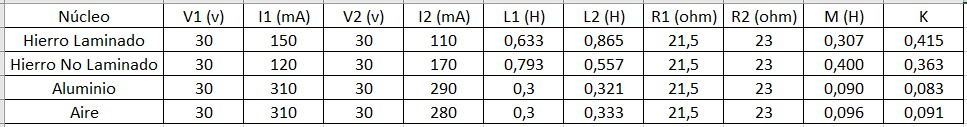
\includegraphics[width=\linewidth]{tabla1.jpg}
    \caption{Resultados obtenidos}
    \end{figure}

    \section{Conexión de Resistencia en el Secundario}
\hspace{1cm} En el siguiente experimento, se conectó una resistencia de \textit{Rd} = 200$\Omega$ en el circuito secundario y se midió 
la caída de tensión determinada como V2. Se hizo un análisis de la caída de potencial V2 y tambíen de la corriente que circula
por el circuito secundario, para cada uno de los núcleos utilizados.

\subsection{Mediciones Experimentales}

\begin{figure}[h]
    \centering
    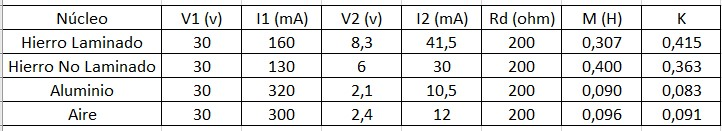
\includegraphics[width=\linewidth]{tabla2.jpg}
    \caption{Resultados obtenidos con Rd conectado en el circuito secundario}
    \end{figure}

\subsection{Análisis de Resultados}
\hspace{1cm} Puede notarse en la tabla anterior, que la caída de tensión en el circuito secundario es mayor cuando se utiliza 
el núcleo


\section{Conclusión}

\end{document}